
\documentclass[12pt,a4paper, twosite]{article}





%\def\numberdoc{\@title} 

%\ifx\conditionmacro\undefined
%\immediate\write18{%
%	pdflatex --jobname="\numberdoc"
%	"\gdef\string\conditionmacro{1}\string\input\space\jobname"
%}%
%\expandafter\stop
%\fi

\usepackage[utf8]{inputenc}
\usepackage[T1]{fontenc}
\usepackage{graphicx}
\usepackage{grffile}
\usepackage{longtable}
\usepackage{wrapfig}
\usepackage{rotating}
\usepackage[normalem]{ulem}
\usepackage{amsmath}
\usepackage{textcomp}
\usepackage{amssymb}
\usepackage{capt-of}
\usepackage{hyperref}
\usepackage[left=2.00cm, right=2.50cm, top=2.50cm, bottom=2.00cm]{geometry}
\usepackage{fancyhdr}
\usepackage[spanish]{babel}
\fancyhead[RO,LE]{\thepage}
\fancyhead[LO]{\emph{\uppercase{\leftmark}}}
\fancyfoot{}
\renewcommand{\headrulewidth}{1.0pt}
\pagestyle{fancy}
\date{\today}

\author{Gastón Valdez \\ gaston.cb.90@gmail.com}
\title{Telemetría y sistema de posicionamiento de antena para interferometría }


\hypersetup{
	pdfborder={0 0 0},
	pdfauthor={Gastón Valdez},
	pdftitle={Reqerimientos de ingenieria de software},
	pdfkeywords={Requerimientos, posicionador de antena},
	pdfsubject={hola mundo},
	pdfcreator={Emacs 26.2 (Org mode 9.1.9)}, 
	pdflang={Spanish}
}


\begin{document}
\begin{titlepage}
\maketitle 
\centering \LARGE Especificación de requerimientos de software. 

\end{titlepage}

\section*{Historial de cambios  }
\begin{tabular}{|c|c|c|}
\hline 
Revisión & Detalles de cambios & Fecha  \\ \hline
A & Creación del documento & 17/3/2022 \\ \hline
B & Corrección de requerimientos &10/4/2022 \\ \hline
C & Se añaden dos requerimientos por pedido del director & 11/4/2022\\ \hline 
D & Entrega de documentación a la catedra de IdS & 11/4/2022 	\\ \hline 

\end{tabular}



\newpage
	\tableofcontents	
\newpage
	\section{Introducción}
	\label{sec:org60390fa}
	En este trabajo aún existen incertezas con respecto a la elección del SBC. Esta situación crea requerimientos incompletos y la conexión de los periféricos con el SBC no se han definido, por este motivo esta definición no se encuentra dentro de los requerimientos de interfaces. 
	\subsection{Propósito}
	\label{sec:org434c3ef}
	Este documento presenta la especificación de SRS para el sistema de  posicionamiento de antena del IAR. Este dispositivo generalmente se conoce como rotador, de dos grados de libertad, uno denominado azimuth y otro altura o elevación.  
	
	Esta dirigido a técnicos, profesionales y operarios que intervengan en los sistemas de apuntamiento que posee el IAR.   

	
	
	\subsection{Ámbito del sistema}
	\label{sec:org12e44a1}
	Este sistema es un subsistema del interferómetro MIA [\ref{ref:MIA}] y el proyecto de construcción de estaciones terrenas. Se objetivo es realizar el apuntamiento de radiofuentes, y el seguimiento de satelites en forma automática.  El nombre del sistema rotador sera ROT\_IAR. el diseño del subsistema ROT\_IAR deberá ser escalable para una posterior etapa de producción.
	
	
	\subsection{Definiciones, Acrónimos y Abreviaturas}
	\label{sec:orgb158e36}
	\begin{enumerate}
		\item IAR: instituto Argentino de Radioastronomía.  
		\item SRS: Especifición de requerimientos de software.  
		\item EP: Electrónica de potencia.
		\item SBC: Single Board Computer.
		\item TBC: Falta de confirmación.
		\item TBD: Aún no definido.
		  
		
	\end{enumerate}
	
	
	
	\subsection{Referencias}
	\label{sec:org62711e0}
	\begin{enumerate}
		\item \label{ref:MIA}https://www.iar.unlp.edu.ar/slider/observatorio/
		\item \label{ref:ptr} Plan de trabajo CESE.
		\item \label{ref:ptr} IAR-OBS-MIA-REQ-R05 (documento interno).
\end{enumerate}
	
	\subsection{Visión general del documento}
	\label{sec:orgdaca22c}
	
	Este documento se realiza siguiendo el estándar IEEE Std. 830-1998 de acuerdo con los lineamientos de la 
	materia Ingeniería de Software de la carrera de especialización de sistema embebidos.
	
	
	\section{Descripción general del documento}
	\label{sec:orgc1c4017}
	
	\subsection{Perspectiva del producto}
	\label{sec:org24980a8}
%	El proyecto aquí especificado es independiente de otros sistemas y no tiene relación con otros productos
	El software es parte de un sistema mayor y común a dos proyectos: MIA y estaciones terrenas. Este sistema de apuntamiento, se adicionara al sistema mecánico de la antena que esta en fase de construcción. El sistema realiza el apuntamiento de antena y podrá ser automático o manual. El diagrama en bloques del sistema se muestra en la figura \ref{fig:diagramaBloques}. 
	
	 El presente documento describe los requerimientos de software del bloque single board computer(TBD), y las interfaces del sistema que se observa en la figura  \ref{fig:diagramaBloques}. 
	\begin{figure}[h!]
		\centering
		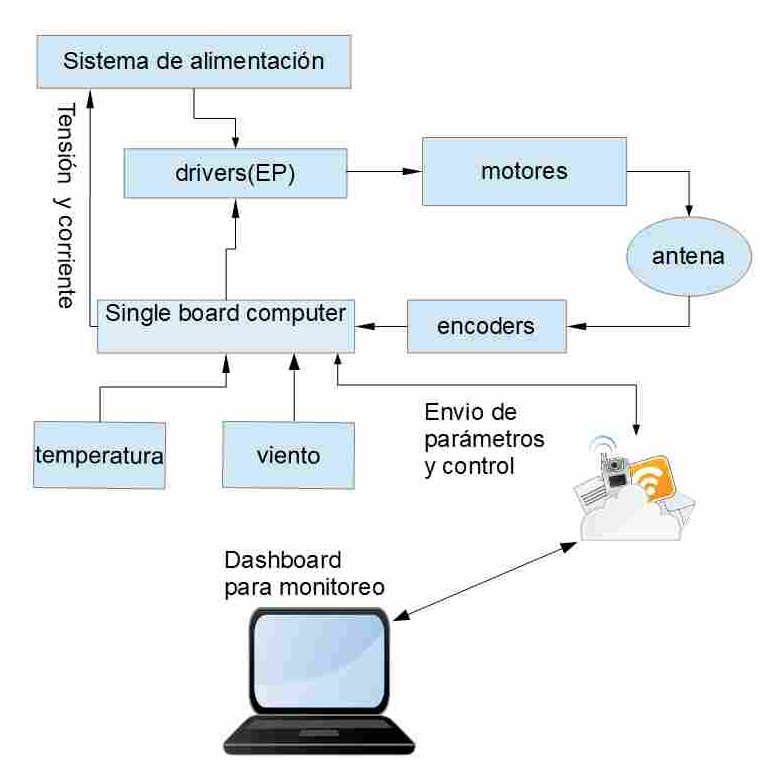
\includegraphics[scale=0.5]{bloquesInt.jpg}
		\caption{Diagrama en bloques del sistema}
		\label{fig:diagramaBloques}
	\end{figure}
	\subsection{Funciones del producto}
	\label{sec:orgaf51da6}
	\begin{enumerate}
		\item Control de posición.
		\item Servidor web embebido. 
		\item Compatible con el software Gpredict y Stellarium, y scripts de antenas principales. 
		\item Reinicio del single board computer en forma remota(TBC).  
		\item Interrupción de operación en caso de condiciones climáticas adversas. 
		\item Información de la operación y estado actual del sistema(tracking, untracked, y cenit). 
	\end{enumerate}
	
	\subsection{Características de los usuarios}
	\label{sec:orga40b0ee}
	Los usuarios serán técnicos, operarios y profesionales con conocimiento y experiencia en los sistemas de apuntamiento y manejo de rotadores. 
	\subsection{Restricciones}
	\label{sec:org5ca5790}
	
	
	\begin{itemize}
		
		\item Lenguaje python 3 para guardar compatibilidad con los scripts de manejo principal de las antenas Carlos Varsavsky y Esteban Bajaja(\ref{ref:MIA}).
		\item El software debe estar bajo control de versiones.  
		\item La documentación se corresponderá con el formato del IAR y con el sistema de numeración del mismo.  
		
%		\item  se debe realizar un informe de avance por cada requerimiento que se cumple 
	\end{itemize}
	
	
	\subsection{Suposiciones y dependencias}
	\label{sec:org0ae23fe}
	\begin{enumerate}
	\item Se supone que se cuenta con los scripts del manejo de las antenas principales.
	\item	Se cuenta con los encoders y motores seleccionados.
	\end{enumerate}
	
	
	
	\subsection{Requisitos futuros}
	\label{sec:org33cfcdb}
	El sistema posea control de velocidad 
	
	El diseño electrónico escalable y realizable en una cadena de producción.  
	
	El sistema debe poseer autocalibración en base al sol o la luna (esto dependerá del horario en que se realice la autocalibración).  
	
	El sistema tendrá que identificarse mediante algún código alfanumérico para brindar sistema de reconocimiento en técnicas de interferometría. 
	
	
	\section{Requisitos específicos}
	\label{sec:org40573d1}
	
	
	\subsection{Interfaces externas}
	\label{sec:orgfd5391f}
	\begin{itemize}
		\item El sistema se comunicara con una red local mediante cable ethernet con conector RJ45[IAR-OBS-MIA-INT-REQ0001] .
		\item El sistema se conecta con un sensor de temperatura DHT11 [IAR-OBS-MIA-INT-REQ0002]. 
		\item El sistema se conecta con los drivers de los motores mediante puertos que posean salida PWM. La velocidad,frecuencia, y porcentaje del PWM será determinado por los ensayos correspondientes sobre los motores[IAR-OBS-MIA-INT-REQ0003].  
		\item Los encoders serán conectados en un puerto analógico digital, o bus de comunicación, sujeto a disponibilidad del mercado local del Single Board Computer[IAR-OBS-MIA-INT-REQ0004]. 
		\item El sistema de medición del viento se realizará con un anemómetro, y se conectará a un puerto analógico digital del Single Board Computer [IAR-OBS-MIA-INT-REQ0005]
		\item Se realizará un PCB que se acople al Single Board Computer mecánicamente con borneras donde se indique mediante serigrafia la conexión de los perifericos. Esta serigrafia será[IAR-OBS-MIA-INT-REQ0006]: 
		\begin{itemize}
			\item EP1: motor de azimuth 
			\item EP2: motor de altura
			\item ENC1: encoder de azimuth 
			\item ENC2: encoder de altura 
			\item VTO: anemómetro 
			
		\end{itemize} 
		
	\end{itemize}
	
	\subsection{Funciones}
	\label{sec:org307bb59}
	\subsubsection{Control de posición}
	\begin{enumerate}
		\item El sistema debe realizar un control a lazo cerrado mediante la lectura de los encoders cada 100 ms en modo automático[IAR-OBS-MIA-FNC-REQ0001]. 
		\item Debe  manejar el sistema de coordenadas ecuatorial y altacimutal y realizar las transformaciones matemáticas correspondientes[IAR-OBS-MIA-FNC-REQ0002]. 
		\item El control se realiza mediante un control proporcional, integral y derivativo[IAR-OBS-MIA-FNC-REQ0003]. 
		\item El sistema tiene tres estados[IAR-OBS-MIA-FNC-REQ0004]: 
			\begin{enumerate}
				\item TRACKING: seguimiento de satélite o radiofuente. Debe ser independiente del tipo de fuente a seguir.
				\item UNTRACKING: no se esta realizando ningún tipo de seguimiento. 
				\item CENIT: posición de reposo de la antena.
			\end{enumerate}

	\end{enumerate}
	\subsubsection{Servidor Web embebido}
	\begin{enumerate}
		\item El servidor informa de los valores del estado actual(TRACKING, UNTRACKING, CENIT). Además informa el estado de corriente en ampere[A], tensión de operación en volts[V], viento en km/h y temperatura en grados centigrados. La medición de la temperatura y velocidad del viento es en el ambiente donde se encuentre el sistema[IAR-OBS-MIA-SWE-REQ0001]. 
		\item Debe realizar movimientos de la antena a demanda del operador[IAR-OBS-MIA-SWE-REQ0002].
		\item Debe poseer una función de calibración para los encoders e informar su lectura[IAR-OBS-MIA-SWE-REQ0003]. 
		\item Debe poseer mecanismo de POST/GET para consulta de estados mediante consola[IAR-OBS-MIA-SWE-REQ0004]. 
		\item Se deben utlizar los scripts de las antenas principales. Esto implica la realización en python del servidor web embebido[IAR-OBS-MIA-SWE-REQ0005].
		\item Debe poseer mecanismo para realizar el gráfico de tensión,corriente, viento y temperatura, durante los últimos 10 minutos y verse en pantalla[IAR-OBS-MIA-SWE-REQ0006].
	\end{enumerate}

\subsubsection{Conexión con software externo}
	\begin{itemize}
		\item Debe usarse Stellarium y Gpredict para realizar seguimientos de radiofuentes o satelites
		\item Se deben utilizar sockets y configuraciones especificas para cada software. 
	\end{itemize}


\subsection{Entorno de operación y mantenimiento}
\begin{enumerate}
	\item El sistema debe realizar la medición de temperatura y viento cada 2 minutos 
	\item Si la velocidad supera los 50 km/h durante diez minutos, debe llevar la antena a su posición de cenit, independientemente de su estado actual. Si estaba en cenit, debe quedarse allí hasta que la velocidad del viento sea inferior a 50 km/h durante al menos 10 minutos[IAR-OBS-MIA-OPM-REQ0001]
	\item Debe almacenar los datos desde las 5AM de un día, hasta las 5AM del día siguiente, y enviar la información a un servidor dentro de la institución. Estos datos tienen el siguiente formato[IAR-OBS-MIA-OPM-REQ0002]: 
	\begin{itemize}
		\item timestamp , tensión[V], corriente[A], temperatura[°C] , viento[KM/H], ESTADO, posición\_azimuth,posición\_altura 
	\end{itemize}  
	La hora de envío será las 5 AM de cada día. El nombre del archivo enviado es en formato txt, y posee el siguiente formato de nombre: 
	\begin{itemize}
		\item IAR\_MIA\_FECHA\_ANTENA.txt 
	\end{itemize} 
	\item El archivo debe ser procesado y almacenado en un directorio dentro del repositorio de la institución mediante un script y realizar un análisis de los parámetros que reciben. En caso de anomalía, debe alertar a los operadores mediante el envío de un SMS o mail[IAR-OBS-MIA-OPM-REQ0003].  
\end{enumerate}

	\subsection{Requisitos de rendimiento}
	\label{sec:org94bc543}
	
	El sistema, debe soportar hasta 20 conexiones simultaneamente. Si esta en estado TRACKING, al conectarse simultaneamente otro operador, debe informarsele que debe esperar que finalice la operación[IAR-OBS-MIA-OTH-REQ0001]. 
	
	\subsection{Restricciones de diseño}
	\label{sec:org49fe900}
	\begin{enumerate}
		
	\item debe realizar el servidor web embebido en python, para tener compatibilidad con los scripts de manejo de las antenas principales de la institución[IAR-OBS-MIA-OTH-REQ0002]. 
	\item Los encoders deben tener una resolución menor a 0.2º(diez veces menor que el ancho de haz de antena) [IAR-OBS-MIA-OTH-REQ0002]. 
	\end{enumerate}

	\subsection{Atributos del sistema}
	\label{sec:orgd0babc0}
	Debe tener la capacidad de actualizar el software manualmente mediante red local, si se desea agregar otro software aparte de Gpredict y Stellarium (por ejemplo orbitron)
	
\section{Apéndices}
\label{sec:org75cea03}
	
\subsection{caso de uso 1 }


%1989C2 cyan 
\begin{tabular}{|p{0.001\textwidth}|p{0.2\textwidth}|p{0.2\textwidth}|p{0.5\textwidth}|}

\hline 
\multicolumn{4}{|p{\textwidth}|}{ Nombre del caso de uso} \\ \hline 
 & Descripción & \multicolumn{2}{|p{0.7\textwidth}|}{ Descripción del caso de usos}  \\ \hline 
 & Actor Principal & \multicolumn{2}{|p{0.7\textwidth}|}{Actor principal}  \\ \hline  
 & Disparadores & \multicolumn{2}{|p{0.7\textwidth}|}{ Disparadores}  \\ \hline 
 & &  \multicolumn{2}{|p{0.7\textwidth}|}{ Descripción del caso de usos}  \\ \hline  
%consultar si unir las dos filas ! 

\multicolumn{4}{|p{\textwidth}|}{ Flujo de eventos} \\ \hline 
& Flujo básico &\multicolumn{2}{|p{0.7\textwidth}|}{ Descripción del flujo, puede usarse newline}  \\ \hline  
% consultar si hay que unir las filas 
& Flujo alternativo   &  \multicolumn{2}{|p{0.7\textwidth}|}{ Flujo alternativo}  \\ \hline  

 
\multicolumn{4}{|p{\textwidth}|}{ Requerimientos especiales } \\ \hline 
&  & \multicolumn{2}{|p{0.7\textwidth}|}{ Ver que aplica y que escribir}  \\ \hline  




\multicolumn{4}{|p{\textwidth}|}{ Pre-condiciones } \\ \hline 
&  & \multicolumn{2}{|p{0.7\textwidth}|}{ Ver que aplica y que escribir}  \\ \hline  


\hline 
\multicolumn{4}{|p{\textwidth}|}{ Post-condiciones } \\ \hline 

&  & \multicolumn{2}{|p{0.7\textwidth}|}{ Ver que aplica y que escribir}  \\ \hline  



\end{tabular}








\subsection{caso de uso 2 }

\subsection{caso de uso 3 }

\subsection{caso de uso 4 }

	
	
\end{document}